% !TEX root = ../main.tex
\section{Translation}
\subsection{Design}
The translator was designed to output the sequence CUAGACUGAAGCUCCUUGAGG, which is the sequence that can activate a FRET tile previously designed in the group. The input was not specifically chosen, but generated by Nupack to fulfill the design parameters. Two versions of the translator were designed, one where the half-translators annealed with 10 bp (\lref{codeshort}), and one where they annealed with 20 bp (\lref{codelong}). The long translator was closer to the setup of the original DNA translator \cite{Picuri2009}, which had annealing lengths of 23-25 bp.

When transcribing the RNA using the T7 RNA polymerase, the sequences are going to start with GG \cite{Milligan1987}, so these were included in the design. Repeats of identical nucleotides were also prevented. The result of the Nupack designed RNA sequences can be seen in \tref{rna_strands} (refer to \fref{translator_short_subunits} and \fref{translator_long_subunits} for strand names).

\begin{figure}[h]
\centering
\includegraphics[width=\textwidth]{figures/translator_short_naming.tikz}
\caption{Sequence naming of the short translator sequences (see table \ref{rna_strands}).}
\label{translator_short_subunits}
\end{figure}


\begin{figure}[h]
\centering
\includegraphics[width=\textwidth]{figures/translator_long_naming.tikz}
\caption{Sequence naming of the long translator sequences (see table \ref{rna_strands}).}
\label{translator_long_subunits}
\end{figure}

To transcribe the RNA sequences, the RNA was converted to DNA, and the T7 promoter was added to the strands. The reverse complement of the strands was found, to serve as the template strand. The T7 RNA polymerase does not need the full template to be double-stranded, only the promoter sequence \cite{Milligan1987}, so the resulting template will be the DNA version of the reverse complement of the target RNA (plus the reverse complement of the promoter), annealed with the promoter sequence (depicted in \fref{rna_to_dna_process}). A program was written to convert the target RNA sequences to their DNA template directly on the output from Nupack, and format it for batch IDT ordering \cite{nupackorder}.

\begin{figure}[h]
\centering
\includegraphics[width=\textwidth]{figures/rna_to_dna.tikz}
\caption{DNA template from RNA sequence for the T7 RNA polymerase.}
\label{rna_to_dna_process}
\end{figure}

\subsection{Transcription}

\begin{table}
\begin{adjustbox}{width=\columnwidth}
\begin{tabular}{llll}
\hline
\textbf{Name}      & \textbf{Short} & \textbf{Sequence}                                           & \textbf{Length} \\
\hline
T7 promoter        & 0          & GGTAATACGACTCACTATAG                                           & 20     \\
Short 1            & 1          & CCTCAAGGAGCTTCAGTCTAGCCCTATAGTGAGTCGTATTACC                    & 43     \\
Short 2            & 2          & CTCCTTGAGGCACATAACTCCCCTATAGTGAGTCGTATTACC                     & 42     \\
Short 3            & 3          & CACATAACTCTACTAAATCTCCCTATAGTGAGTCGTATTACC                     & 42     \\
Short 4            & 4          & GAGTTATGTGCCTCAAGGAGCCCTATAGTGAGTCGTATTACC                    & 42     \\
Short 5            & 5          & AGATTTAGTAGAGTTATGTGCCCTATAGTGAGTCGTATTACC                     & 42     \\
Long 1             & 6          & GTCAATTCGCCTCAAGGAGCTTCAGTCTAGCCCTATAGTGAGTCGTATTACC           & 52     \\
Long 2             & 7          & GCTCCTTGAGGCGAATTGACCCATCTTCATTCTACTCCTACCCTATAGTGAGTCGTATTACC & 62     \\
Long 3             & 8          & CCATCTTCATTCTACTCCTATACCTCAATCCCCTATAGTGAGTCGTATTACC           & 52     \\
Long 4             & 9          & TAGGAGTAGAATGAAGATGGGTCAATTCGCCTCAAGGAGCCCCTATAGTGAGTCGTATTACC & 62     \\
Long 5             & 10         & GATTGAGGTATAGGAGTAGAATGAAGATGGCCCTATAGTGAGTCGTATTACC           & 52     \\
Beacon fluorophore & 11         & CGGCTAGACTGAA                                                  & 13     \\
Beacon quencher    & 12         & CCTCAAGGAGCTTCAGTCTAGCCG                                       & 24 \\
\hline
\end{tabular}
\end{adjustbox}
\caption{Sequences and names of the DNA strands used for transcription.}
\label{dna_strands}
\end{table}

\begin{table}
\begin{adjustbox}{width=\columnwidth}
\begin{tabular}{llll}
\hline
\textbf{Name}      & \textbf{Short} & \textbf{Sequence}                                           & \textbf{Length} \\
\hline
Short 1            & 1          & GGCUAGACUGAAGCUCCUUGAGG                    & 23     \\
Short 2            & 2          & GGGAGUUAUGUGCCUCAAGGAG                     & 22     \\
Short 3            & 3          & GGAGAUUUAGUAGAGUUAUGUG                     & 22     \\
Short 4            & 4          & GGCUCCUUGAGGCACAUAACUC                     & 22     \\
Short 5            & 5          & GGCACAUAACUCUACUAAAUCU                     & 22     \\
Long 1             & 6          & GGCUAGACUGAAGCUCCUUGAGGCGAAUUGAC           & 32     \\
Long 2             & 7          & GGUAGGAGUAGAAUGAAGAUGGGUCAAUUCGCCUCAAGGAGC & 42     \\
Long 3             & 8          & GGGAUUGAGGUAUAGGAGUAGAAUGAAGAUGG           & 32     \\
Long 4             & 9          & GGGCUCCUUGAGGCGAAUUGACCCAUCUUCAUUCUACUCCUA & 42     \\
Long 5             & 10         & GGCCAUCUUCAUUCUACUCCUAUACCUCAAUC           & 32     \\
% Beacon fluorophore & 11         & CGGCTAGACTGAA                                                  & 13     \\
% Beacon quencher    & 12         & CCTCAAGGAGCTTCAGTCTAGCCG                                       & 24 \\
\hline
\end{tabular}
\end{adjustbox}
\caption{Sequences and names of the transcribed RNA strands.}
\label{rna_strands}
\end{table}

The oligos from IDT were dissolved in TE buffer (\tref{te_buffer}) to an approximate concentration of 120 \si{\micro}M, based on the quantity of substance written on the tubes. The final concentration desired was 100 \si{\micro}M, but due to a risk of inaccurate substance quantities, the dissolved concentration was chosen to be slightly above. The oligos could then be further diluted after measuring their absorbance on the Nanodrop.

After dissolving the oligos, the absorbance of each sample was measured on the Nanodrop in triplets. A program was written which can take the .csv output of the Nanodrop, and calculate the concentration based on each strands extinction coefficient \cite{nanodropimport}. The measured concentrations (\fref{oligo_concentrations}) was used to dilute the samples further, to a concentration of 100 \si{\micro}M.

To anneal the templates to the promoter, each of the template strands were mixed with equal amounts of promoter strand in annealing buffer (\tref{annealing_buffer}), to a final concentration of 1 \si{\micro}M. The mixed samples were then heated to 90$^\circ$ C for 5 minutes, and left to cool down to room temperature.

To check if samples annealed properly, they were run on a 20\% native PAGE gel for 3 hours. Each lane was loaded with 50 \si{\micro}l sample, and 10 \si{\micro}l native loading buffer (\tref{native_buffer}). Afterwards the gel was stained in SYBR Gold, and visualised on the Typhoon scanner. The result of the scan can be seen in \fref{promoter_annealing_gel}.

\begin{figure}[h]
\begin{subfigure}[t]{0.54\textwidth}
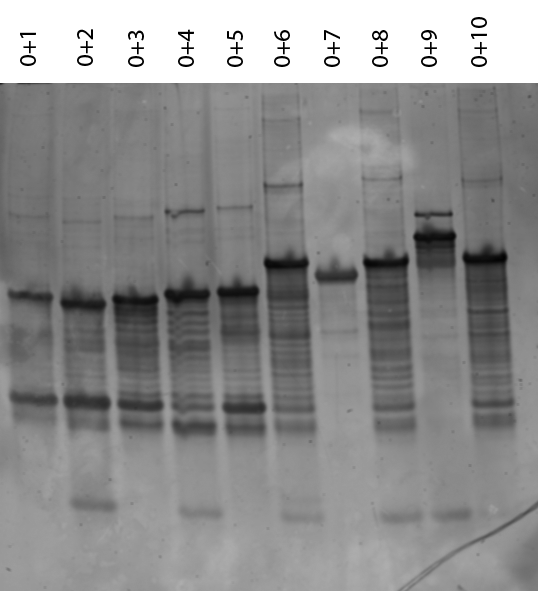
\includegraphics[width=\textwidth]{images/promoter_annealing_gel.png}
\caption{}
\label{promoter_annealing_gel}
\end{subfigure}
\begin{subfigure}[t]{0.46\textwidth}
  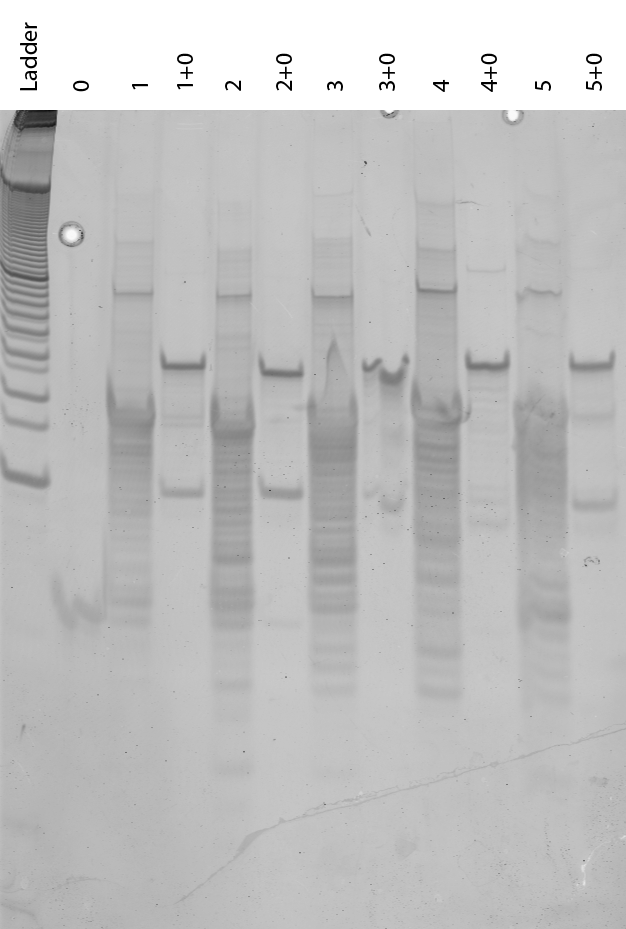
\includegraphics[width=\textwidth]{images/translator_annealing_2.png}
  \caption{}
  \label{translator_annealing_2}
\end{subfigure}
\caption{\subref{promoter_annealing_gel} Typhoon scan of SYBR Gold stained native PAGE gel, with the annealed templates and promoter strands. The lanes are labelled by which strands are annealed (see table \ref{dna_strands}). \subref{translator_annealing_2} The annealed oligos together with controls and a 10 nt ladder. The lanes are labelled with the oligo names given in \tref{dna_strands}. The plus symbol denotes which strands are annealed.}
\end{figure}

As can be seen in \fref{promoter_annealing_gel}, the darkest bands are the annealed samples. The samples for the short translator runs as about the same size, while there is bigger variation in the long translator samples, as expected based on \tref{dna_strands}. The exact positions of the long translator samples does not match with the sequence length, though this can be explained by secondary structures of the single-stranded part of the sample. The shorter bands visible below, are probably excess promoter, other secondary structures, and shorter sequences from synthesis errors. No lane with ladder was run, so the exact position of the bands can't be commented on.

To get the desired RNA sequences, a transcription reaction was run with each of the annealed DNA templates, according to \tref{transcription1}. The samples were left overnight at 37$^\circ$ C. The day after, 1 \si{\micro}L of RNAse free DNAse was added to the samples, and heated for 37$^\circ$ C for an hour. Afterwards, 100 \si{\micro}L of denaturing loading buffer was added to each sample, and 10 ul of the DNA 0 and DNA 5 strands (as controls) were mixed with 10 \si{\micro}L of denaturing loading buffer, and heated for 5 minutes at 90$^\circ$ C.

\begin{table}
  \centering
\begin{tabular}{llll}
  \hline
                       & \textbf{Initial conc.} & \textbf{Final conc.} & \textbf{Volume} \\ \hline
  Transcription buffer & 10X                    & 1X                   & 10 \si{\micro}L           \\
  DTT                  & 100 mM                 & 10 mM                & 10 \si{\micro}L           \\
  NTP mix              & 25 mM                  & 2.5 mM               & 10 \si{\micro}L           \\
  Template             & 500 nM                 & 50 nM                & 10 \si{\micro}L           \\
  T7 RNA polymerase    &                        &                      & 1 \si{\micro}L            \\
  Nuclease-free water  &                        &                      & 59 \si{\micro}L           \\
  Total                &                        &                      & 100 \si{\micro}L          \\ \hline
\end{tabular}
\caption{Mixing of compounds for the first transcription done on the templates for both the short and long translater.}
\label{transcription1}
\end{table}

To purify the RNA, the transcribed sequences and controls were run on a 20\% denaturing PAGE gel, for 4 hours at 20 W. The RNA product should be visible in UV shadowing, but no product was seen. The gel was then stained with SYBR Gold and scanned on the Typhoon. As can be seen in \fref{transcription_1}, the gel wasn't stained long enough, so after restaining it in SYBR Gold, it was scanned again.

\begin{figure}[h]
  \begin{subfigure}[t]{0.49\textwidth}
  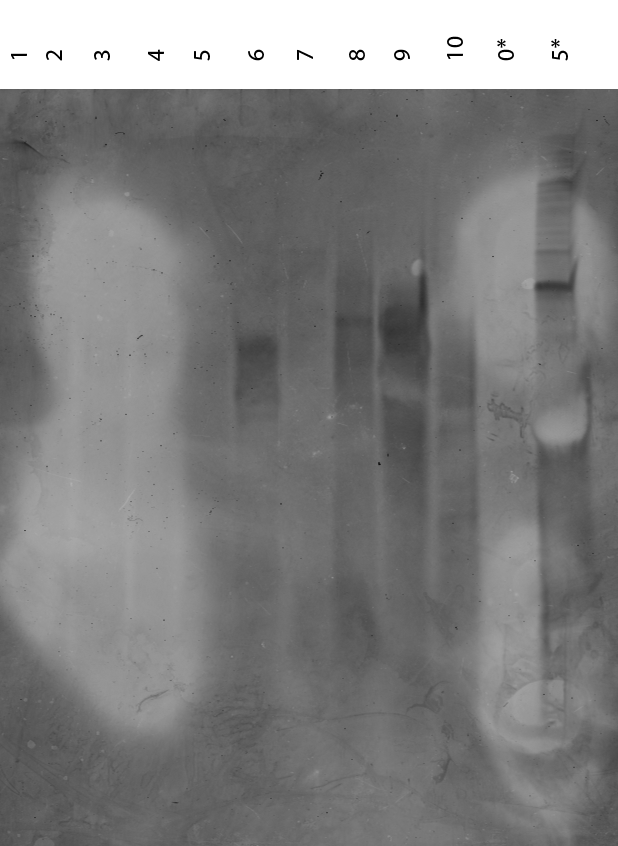
\includegraphics[width=\textwidth]{images/translator_transcription_1.png}
  \caption{}
  \label{transcription_1}
  \end{subfigure}
  \begin{subfigure}[t]{0.49\textwidth}
    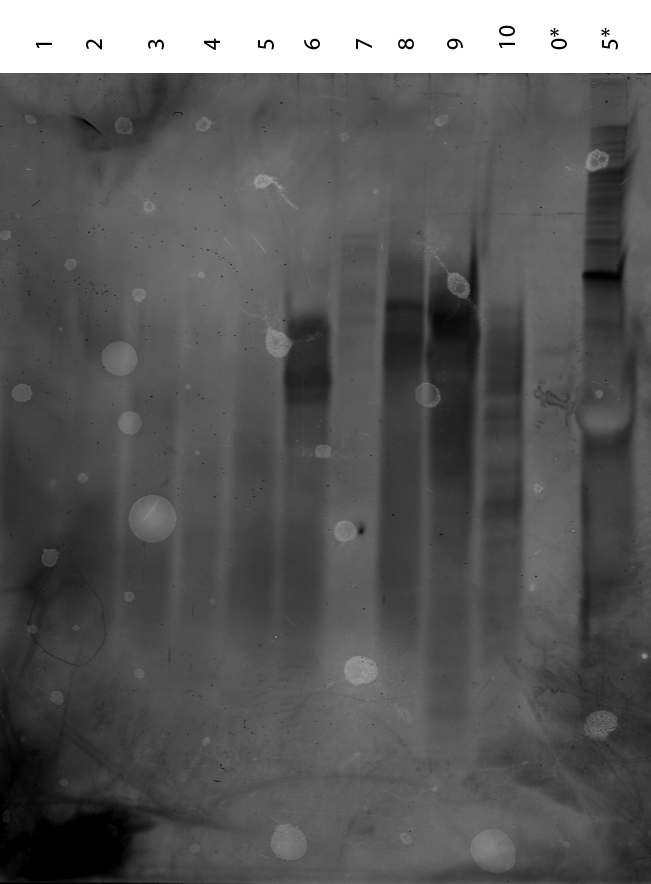
\includegraphics[width=\textwidth]{images/translator_transcription_2.png}
    \caption{}
    \label{transcription_2}
  \end{subfigure}
  \caption{\subref{transcription_1} Typhoon scan of SYBR Gold stained native PAGE gel, with the transcribed RNA strands in lanes 1-10, and controls in 11 and 12. The lanes are labelled by which strands are annealed (see \tref{rna_strands}). The asterix refers to the DNA strands in \tref{dna_strands}. \subref{transcription_2} The same gel after further staining in SYBR Gold.}
\end{figure}

The lanes 1-10 in \fref{transcription_2} does not show distinct bands. There seems to be more product from the long translator transcriptions (lanes 6-10), than in the short ones (lanes 1-5). Even the controls which were loaded in equal amounts does not show up in equal strength. Since the gel from the DNA annealing was run without any controls, it was difficult to see if there was any errors in the annealing. Another 20\% native PAGE gel was run with the annealed DNA, using the single stranded oligos as control. To simplify the experiment while trying to find the error, only the short translator sequences were used.

The results of \fref{translator_annealing_2} still shows that the templates have annealed with the promoter, and runs as about 40-50 bp. The expected size is around 60 bp (sum of promoter and template), but it is difficult to say how a partly annealed structure will run on a native gel. The new gel does however show that the bands in the annealed lanes below the assumed product, might not be excess promoter. The promoter is seen in the second lane, and lies below the bands in the annealed structure thought to be excess promoter. The bands below the product might be due to secondary structures of each of the template strands, but comparing with \fref{short_secondary_structures}, the band in the 5+0 lane would be expected to be less visible, as strand 5 has no secondary structure.

Despite the unexplained bands from the annealing, a new transcription was run on the short template strands to see if better results could be obtained. The transcription was done using the previous protocol, and run on a gel. The UV shadowing still did not show any visible product, so the gel was scanned to check for bands.

\begin{figure}[h]
\begin{subfigure}[t]{.43\textwidth}
  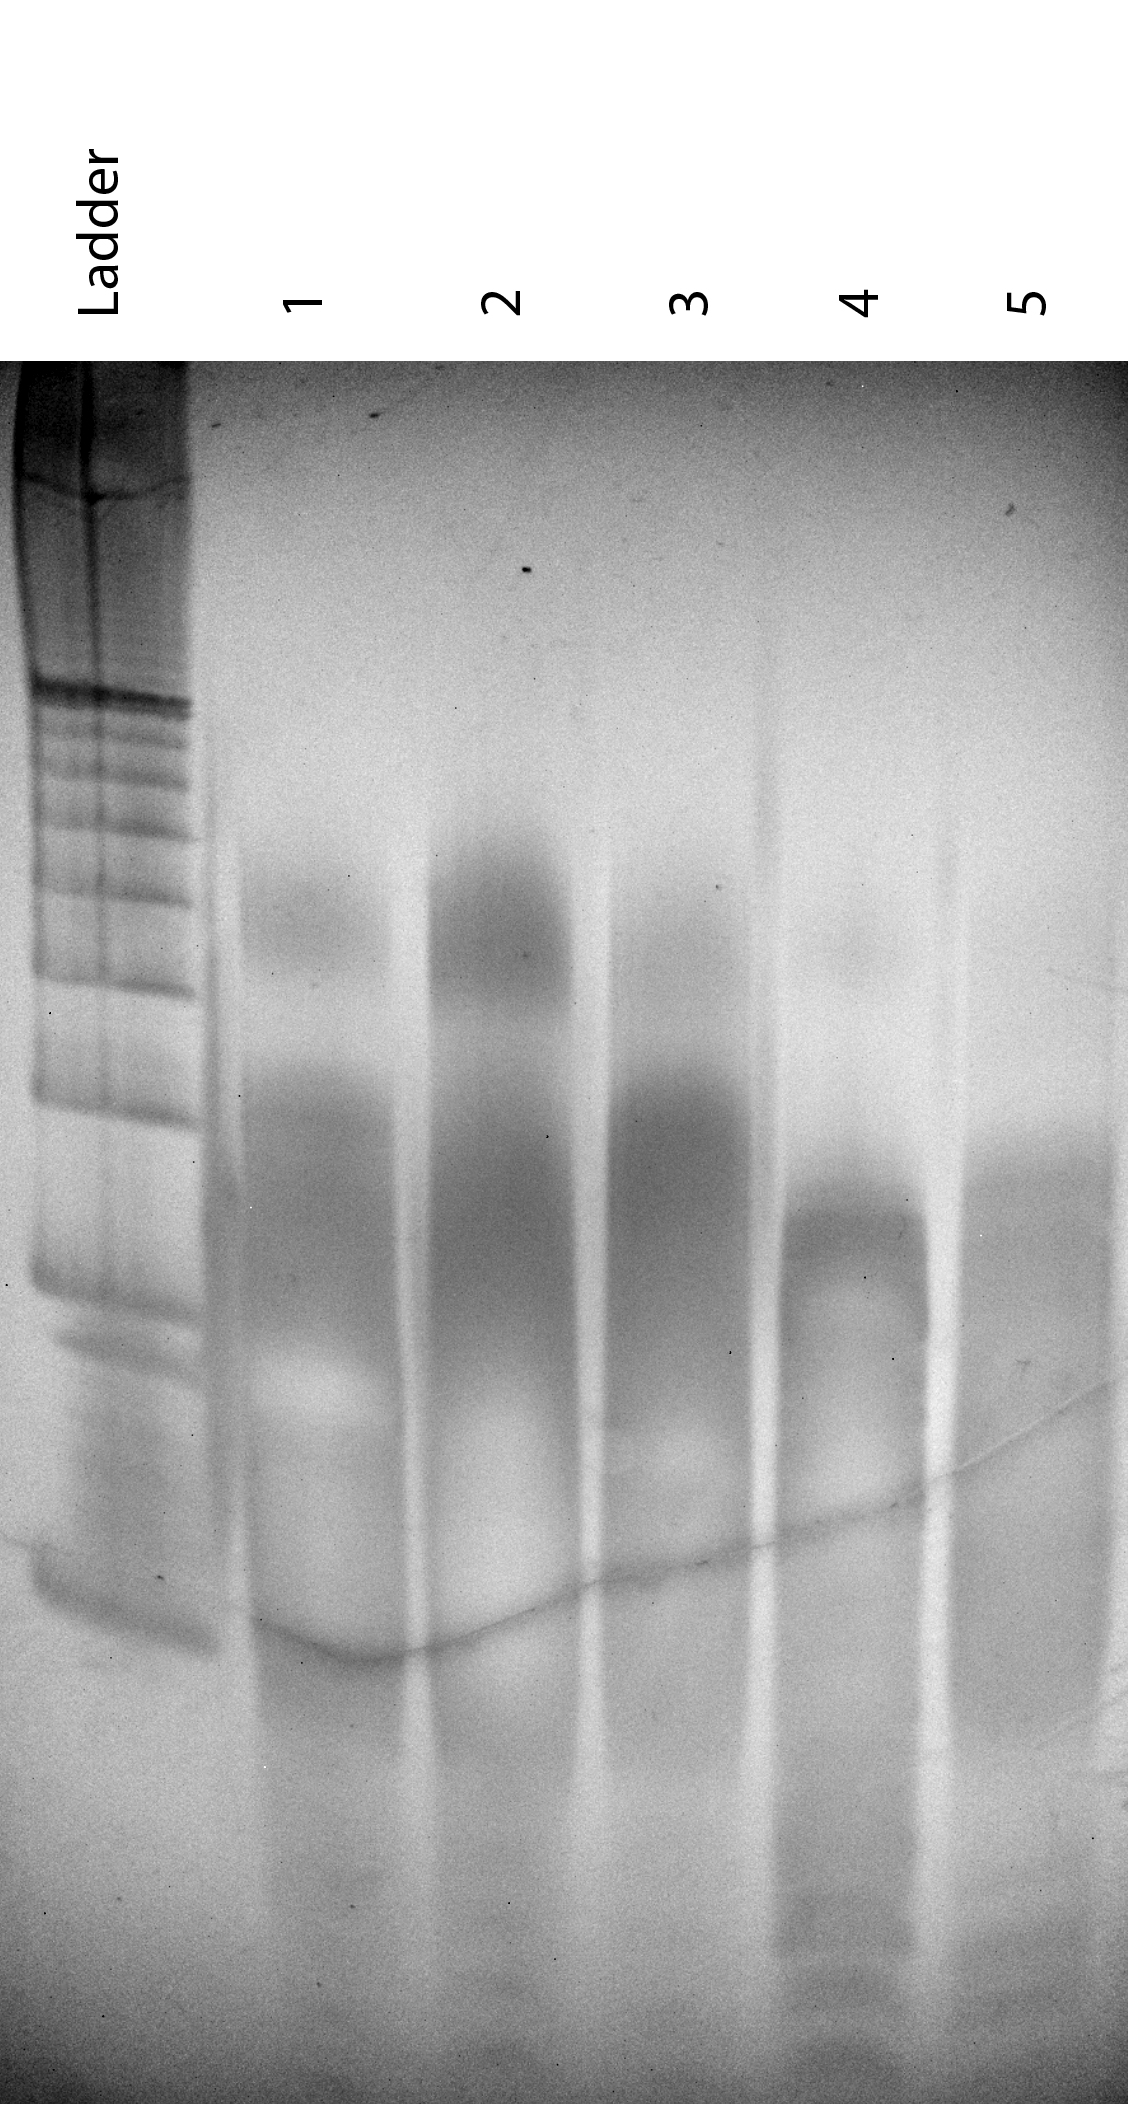
\includegraphics[width=\textwidth]{images/translator_transcription_3.png}
  \caption{}
  \label{translator_transcription_3}
\end{subfigure}
\begin{subfigure}[t]{.55\textwidth}
  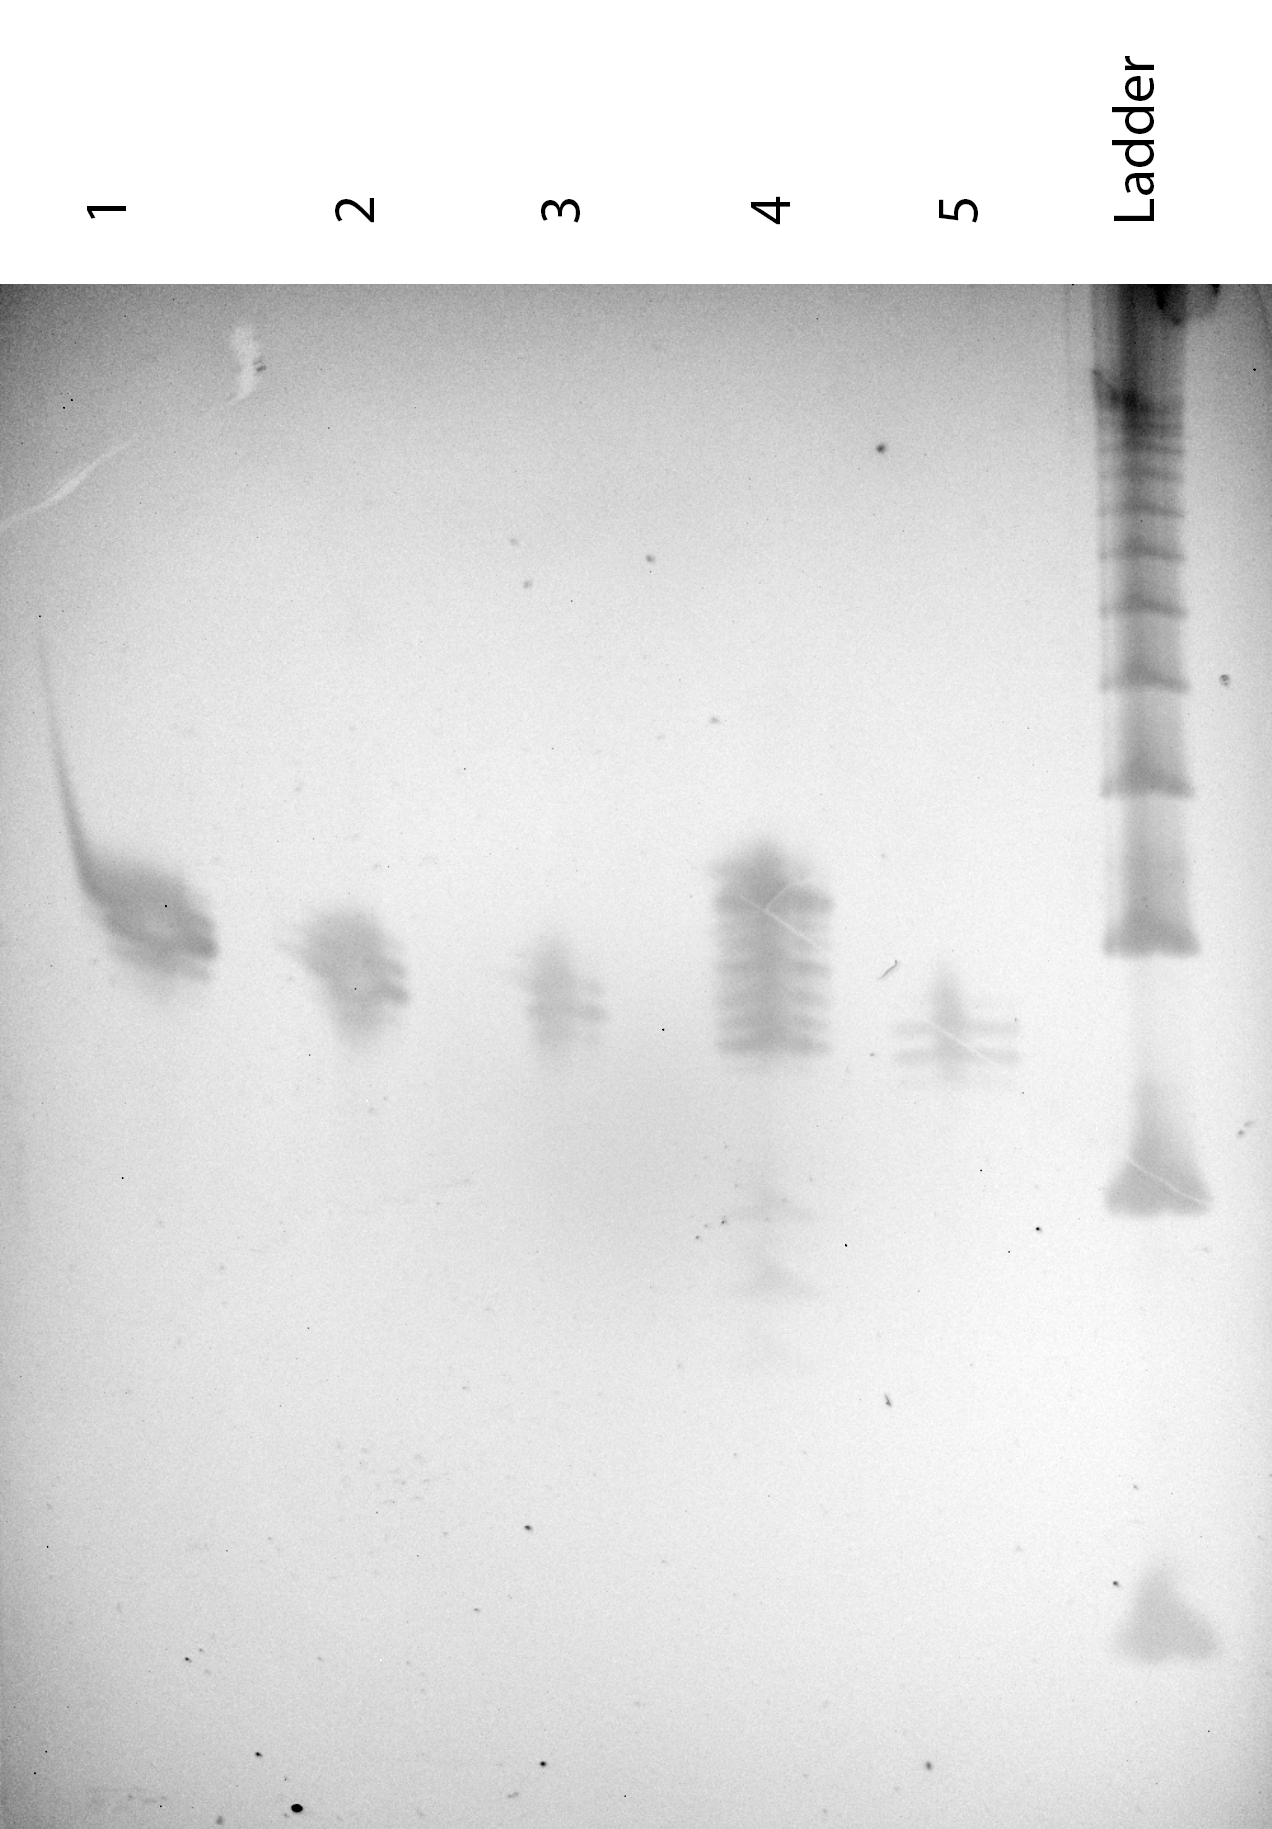
\includegraphics[width=\textwidth]{images/translator_transcription_purified.png}
  \caption{}
  \label{translator_transcription_purified}
\end{subfigure}
\caption{\subref{translator_transcription_3} The transcribed short translator sequences and a 10 nt ladder. The lanes are labelled with the oligo names given in \tref{rna_strands}. \subref{translator_transcription_purified} The purified short translator RNA oligos.}
\end{figure}

As seen in \fref{translator_transcription_3}, still no clear bands with RNA product was visible. After checking all buffers and materials, it was learned that the T7 polymerase that was used was from 2013, and might have been too old to still function properly. A fresh T7 polymerase was used for a new transcription, same as the previous protocol. The UV shadowing did show some distinct bands this time, so the bands were cut out for purification. The purification was done using the precipitation protocol \cite{precipitationprotocol}. After purification the pellets were dissolved in 100 \si{\micro}L TE buffer, their absorbance measured on the Nanodrop, and their concentration calculated using their extinction coefficients.

To check that the purification worked, 2 \si{\micro}L of each sample with 1 \si{\micro}L of denaturing loading buffer was run on a 20\% denaturing gel, stained with SYBR Gold, and visualised on the Typhoon.

\fref{translator_transcription_purified} shows that the RNA has been isolated, but is not very pure. It is possible that when cutting out the RNA from the gel before purification, too large an area was taken. The target RNA sequences were still expected to be in the purified samples (albeit not very pure), and it has previously been shown that strand displacement reactions can work with unpurified components \cite{Thubagere2017}, so the experiment continued with the current RNA.

Based on the concentrations in \fref{translator_transcription_concentration}, the samples were further diluted in RNAse-free water to 2 \si{\micro}M for the translator strands (1-4) and 1 \si{\micro}M for the input strand (5). Then 25 \si{\micro}L of each of the translator strands were mixed with their respective counterpart (1+2 and 3+4) to a final concentration of 1 \si{\micro}M in 50 \si{\micro}L.

At this point, the reporter samples were also mixed and diluted in RNAse-free water to the same concentration as the translator subunits. To each of the subunits and the reporter, 5 \si{\micro}L of 10X annealing buffer was added. The samples were heated at 90$^\circ$ C for 5 minutes, and cooled off at room temperature.

To check if the subunits and reporter annealed properly, they were run on a 20\% native PAGE gel with the single strands as control. It was expected that the fluorophore would be visible at the same wavelength as SYBR Gold, so a scan without staining should show the free fluorophore (and not the quenched fluorophore in the annealed reporter).

\begin{figure}[h]
\begin{subfigure}[t]{.5\textwidth}
  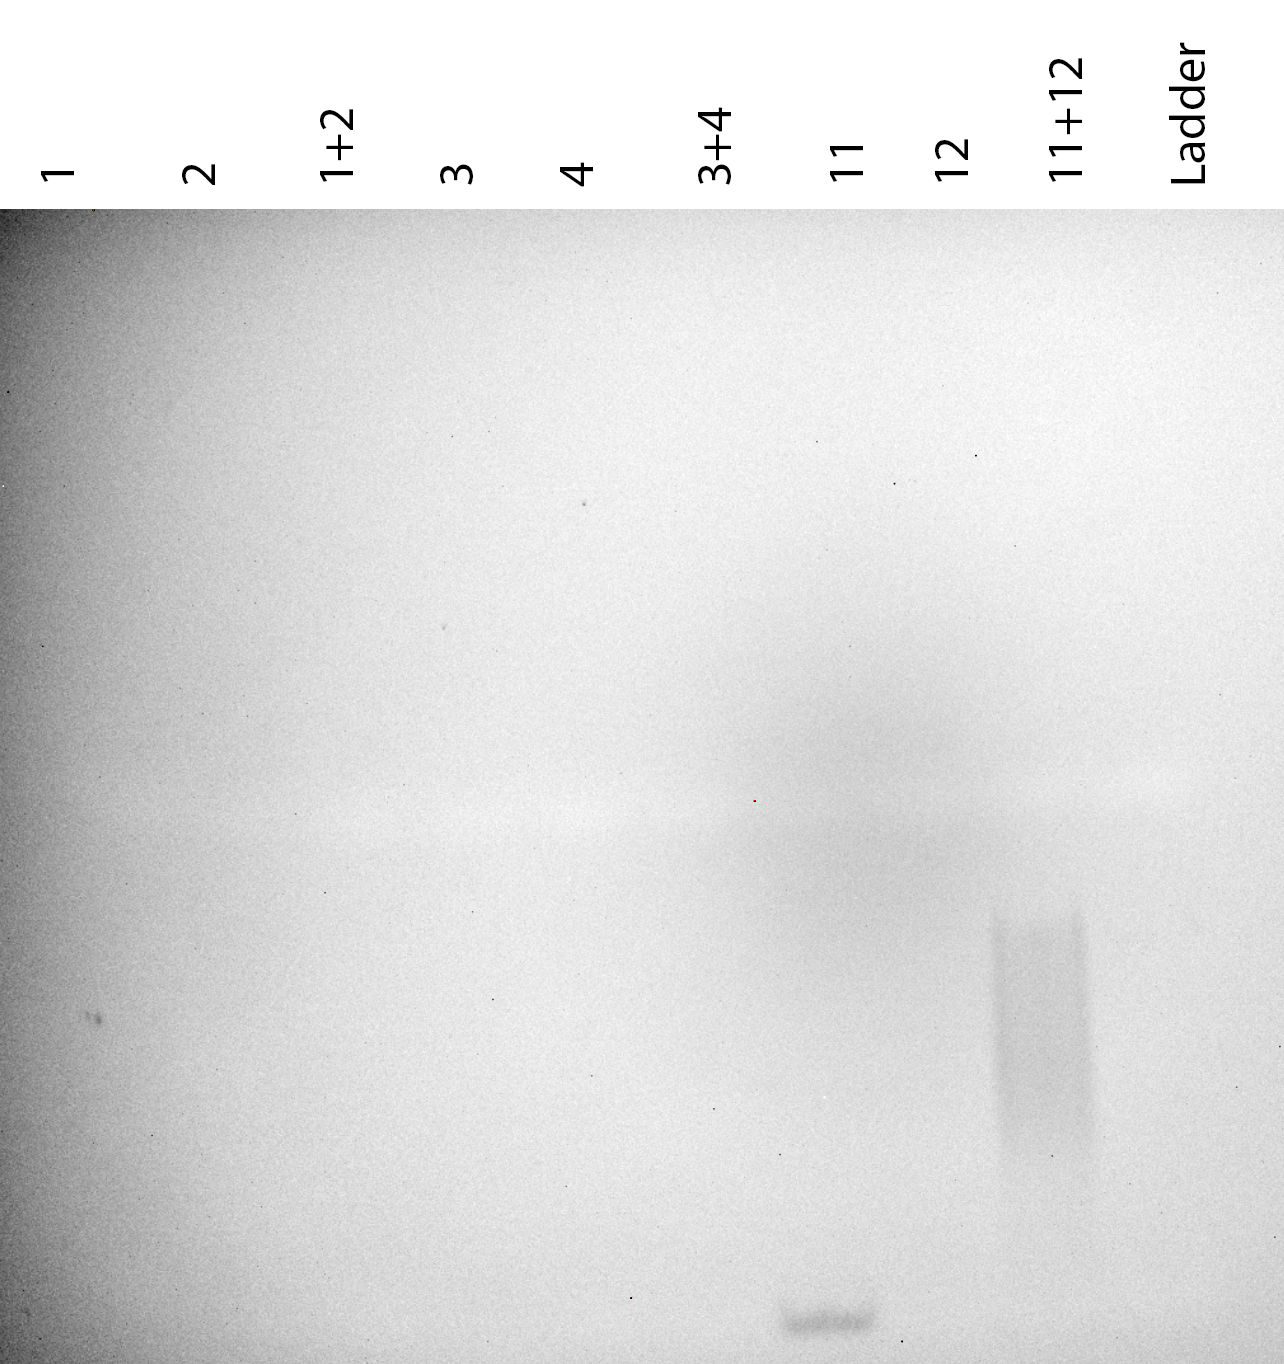
\includegraphics[width=.5\textwidth]{images/transcription_annealed_nostain.png}
  \caption{Not stained}
  \label{transcription_annealed_nostain}
\end{subfigure}
\begin{subfigure}[t]{.5\textwidth}
  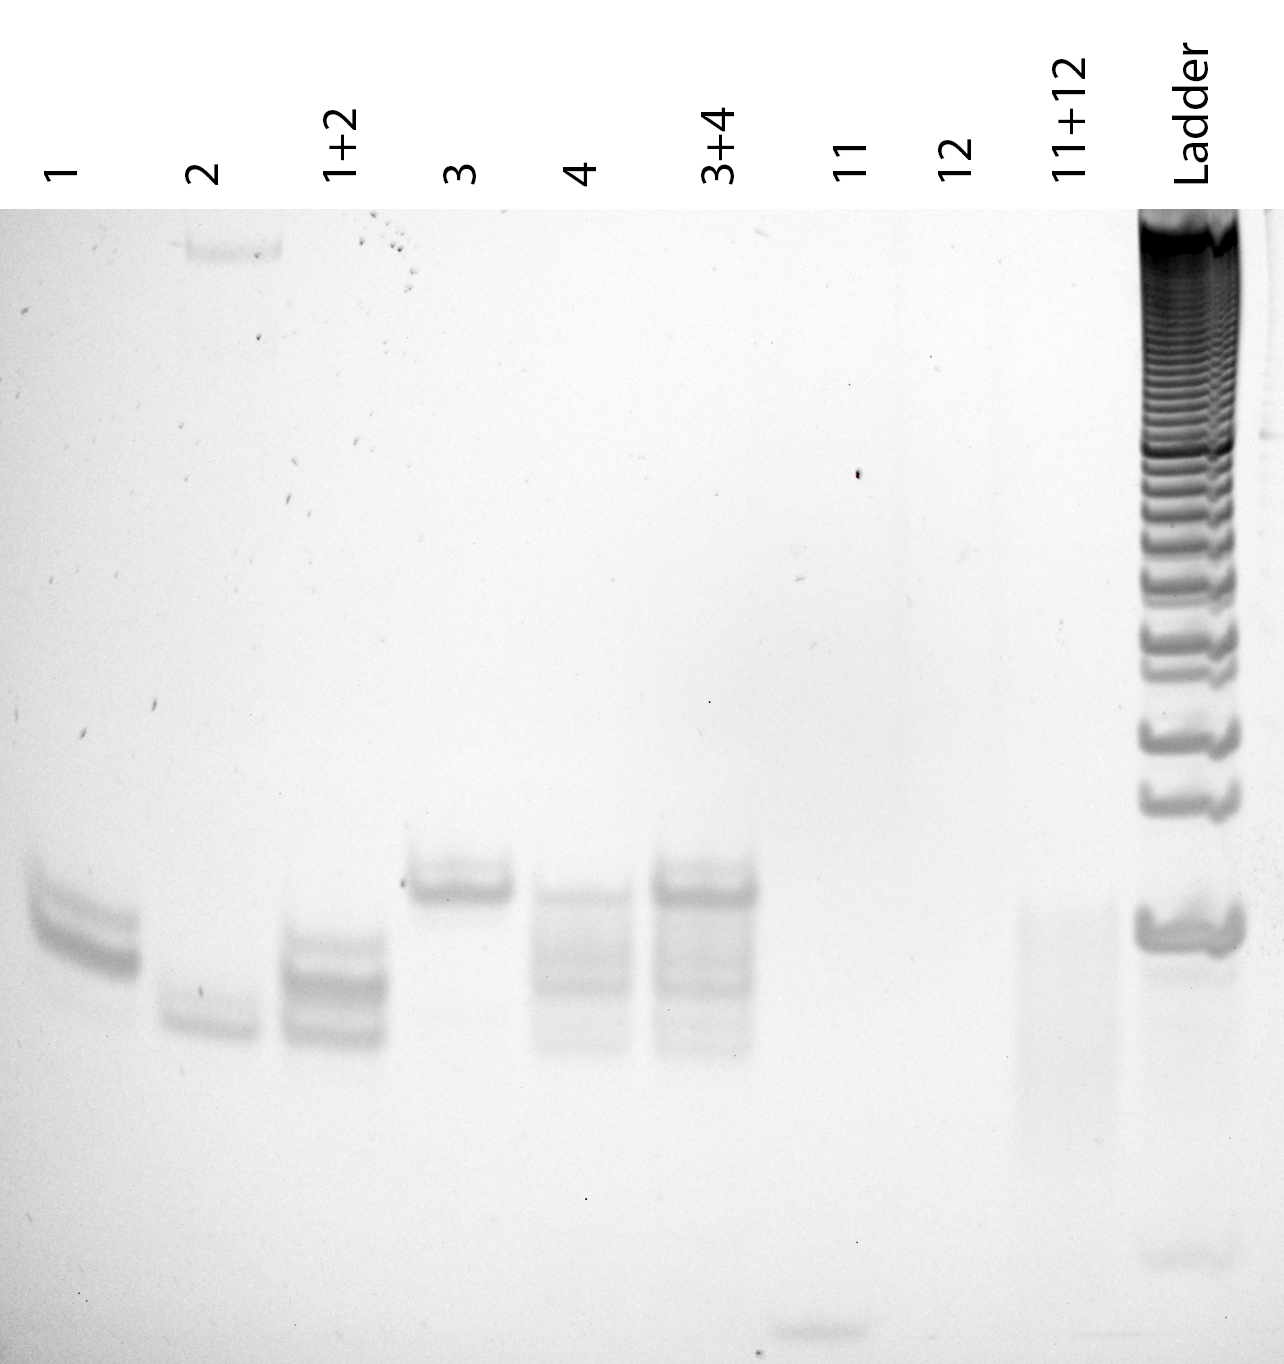
\includegraphics[width=.5\textwidth]{images/transcription_annealed_stain.png}
  \caption{Stained}
  \label{transcription_annealed_stain}
\end{subfigure}
\caption{The annealed short translator subunits and reporter, with the single strands as controls, and a 10 nt ladder.}
\label{transcription_annealed}
\end{figure}

As seen in \fref{transcription_annealed_nostain}, the fluorophore clearly shows up in the unstained scan, and gets partly quenched and moves up when annealed to its quencher. The smear in the annealed reporter might be due to synthesis errors in the quencher strand.

In the stained scan (\fref{transcription_annealed_stain}), the annealed half-translators does not seem to have annealed at all. Comparing with the controls, the strands that was supposed to have annealed, merely looks like the sum of the single strands. There is a few reasons why this could have happened. The RNA that was purified from gel was not the correct sequences, the annealing was not carried out correctly, or the strands simply doesn't anneal very good.

To check the strength of the annealing, the strands were analyzed in Nupack. The result (\fref{annealing_concentration}) shows that the short translator sequences does not anneal as good as the long ones. Due to time constraints, the focus moved towards the long translator sequences, as they were expected to provide better results.

A new transcription for the long translator sequences was prepared using the previous protocol. The transcription was run for 3 hours at 37$^\circ$ C and then run on a 20\% denaturing PAGE gel for 2 hours. No immediate product was visible, but a scan revealed that some RNA had been produced.

\begin{figure}[h]
\begin{subfigure}[t]{0.51\textwidth}
  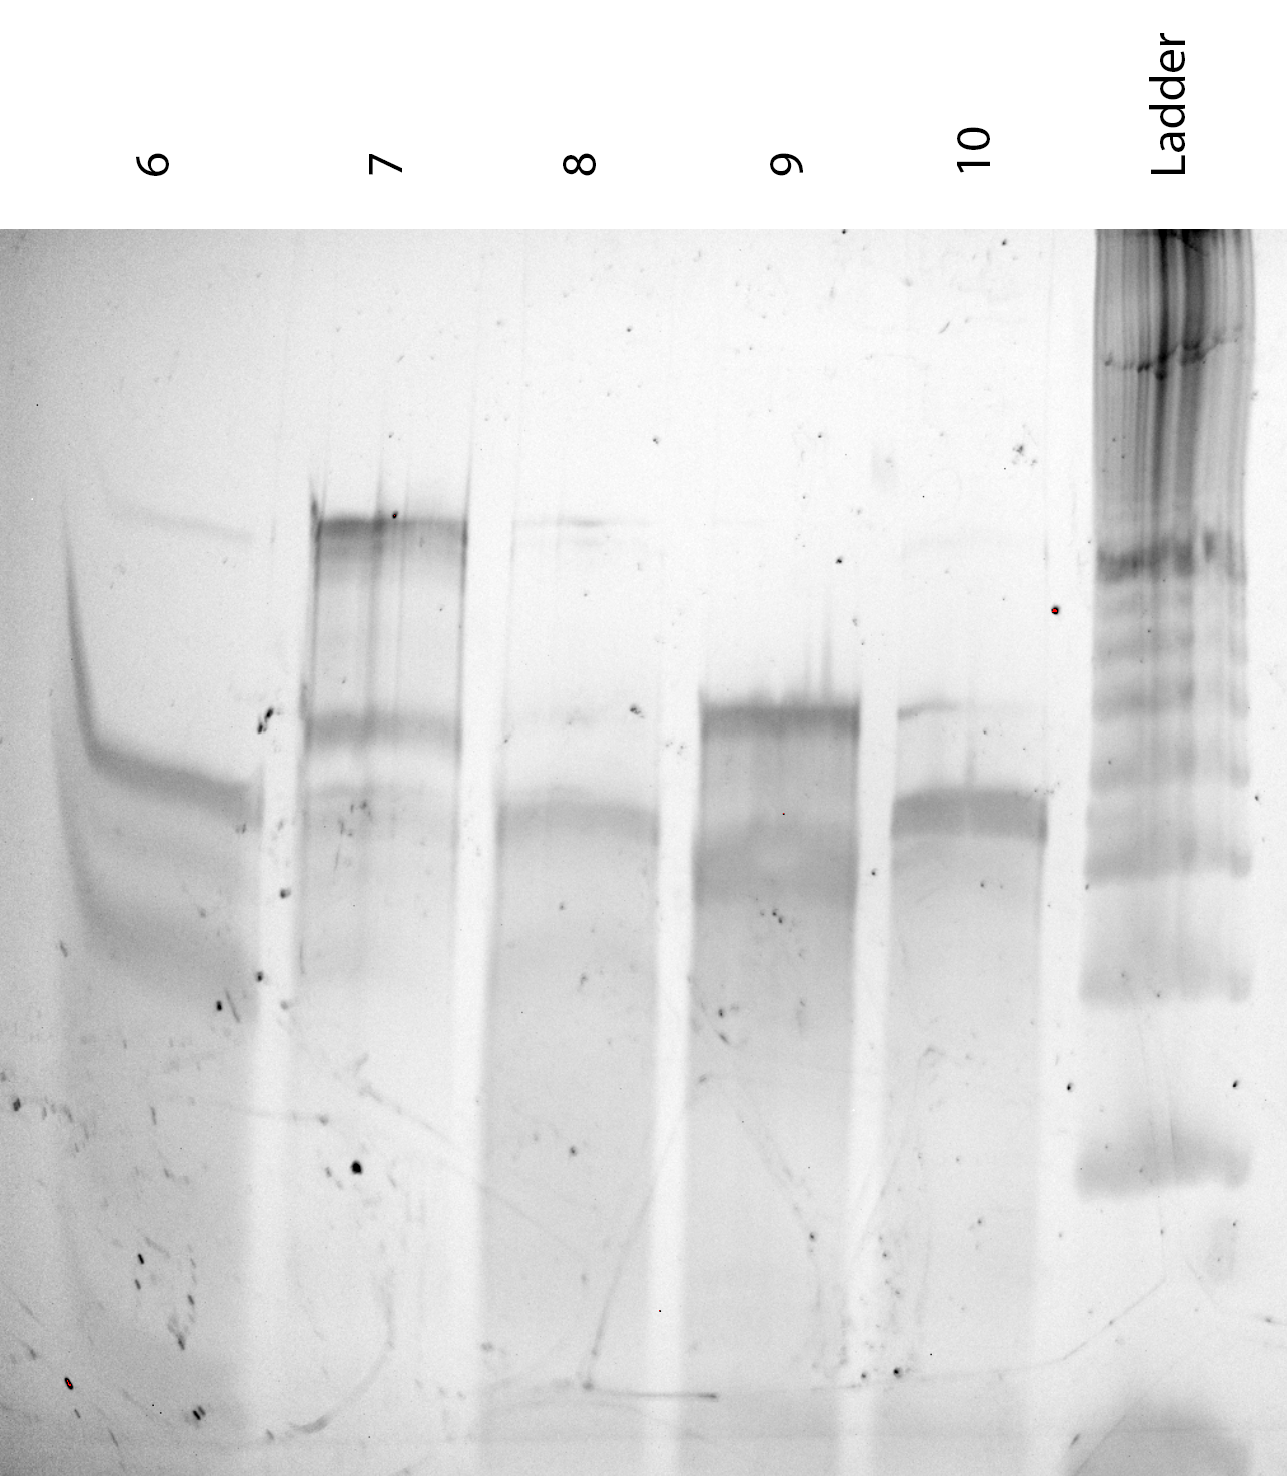
\includegraphics[width=\textwidth]{images/translator_transcription_long_1.png}
  \caption{}
  \label{translator_transcription_long_1}
\end{subfigure}
\begin{subfigure}[t]{0.49\textwidth}
  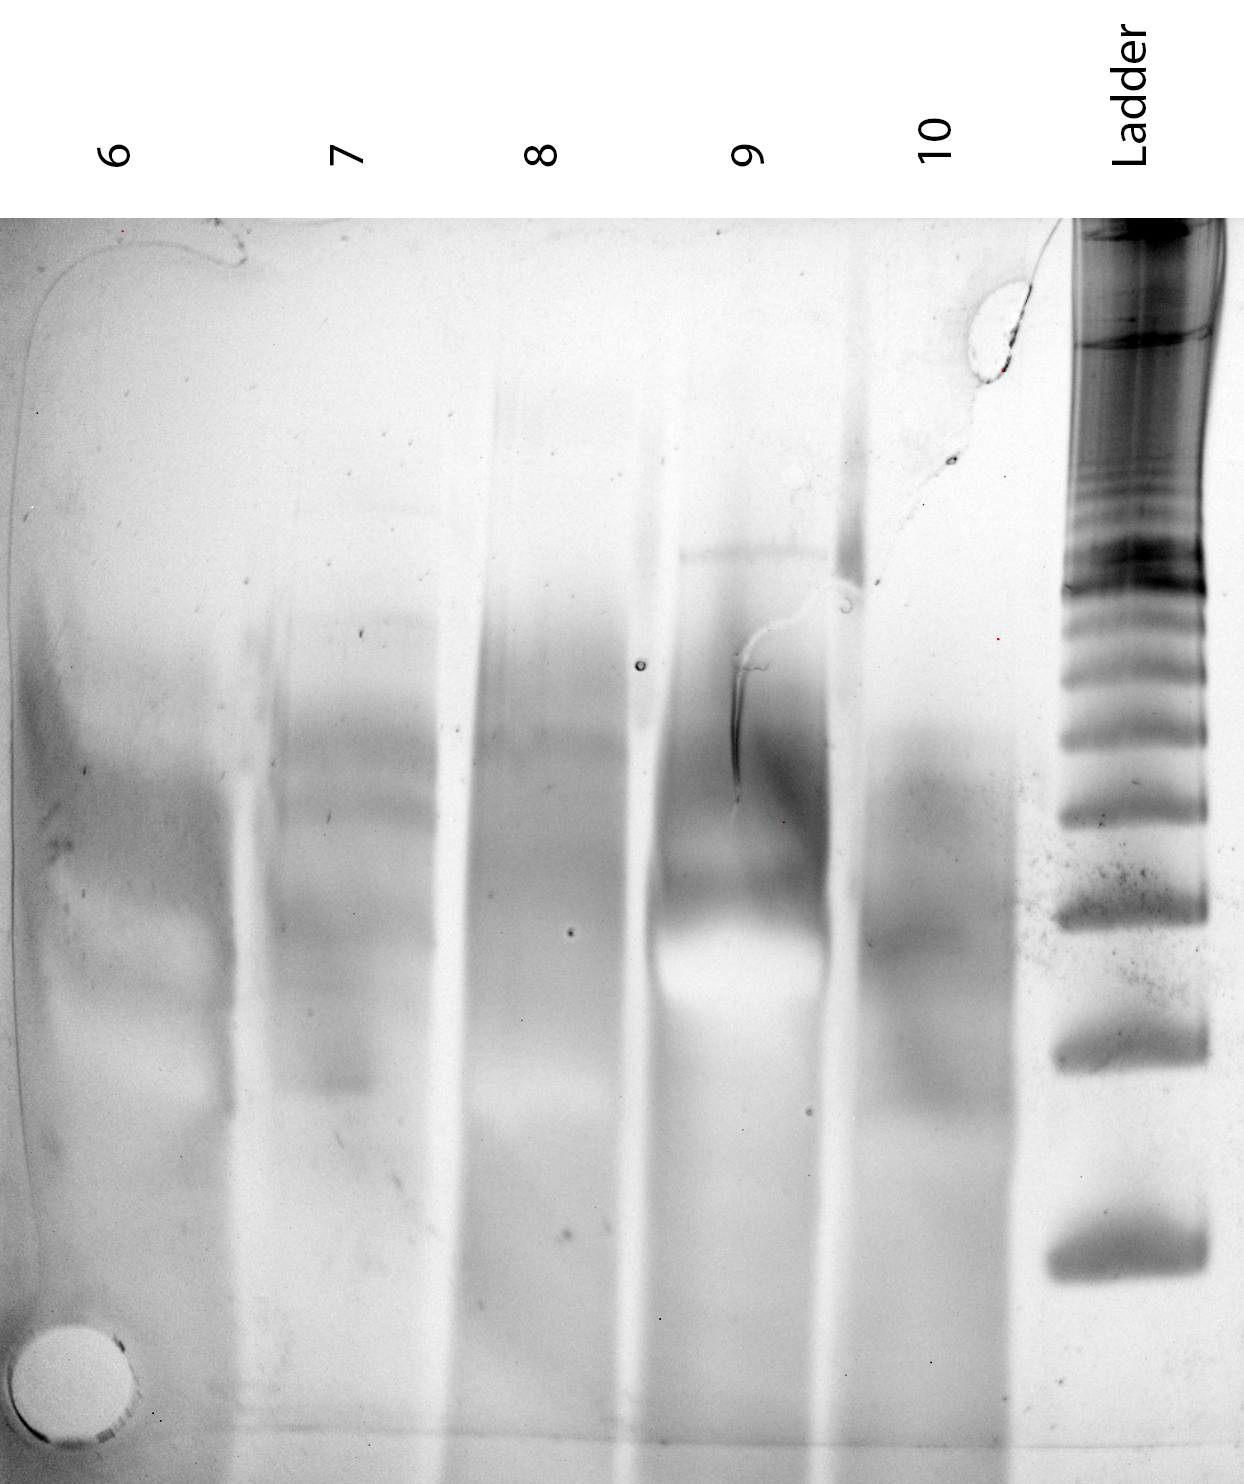
\includegraphics[width=\textwidth]{images/translator_transcription_long_2.png}
  \caption{}
  \label{translator_transcription_long_2}
\end{subfigure}
\caption{\subref{translator_transcription_long_1} Transcription of the long translator sequences with a 10 nt ladder. \subref{translator_transcription_long_2} Transcription of the long translator sequences with a 10 nt ladder, using an adapted protocol.}
\end{figure}

As seen in \fref{translator_transcription_long_1}, some RNA was produced so the concentration of nucleotides in the reaction was increased to get enough RNA to be visible in UV shadowing. The transcription protocol was also changed to one recommended from the supplier of the T7 polymerase \cite{nebtranscription}, to ensure that the polymerase was not the problem (\tref{transcription2}). The new transcription was carried out as the previous one, and revealed a single band (strand 9) in UV shadowing, but the rest of the templates had not produced enough RNA to be purified. A scan revealed once again that RNA had been produced, but the right product could not be isolated.

\begin{table}
\centering
\begin{tabular}{llll}
  \hline
   & \textbf{Initial conc.} & \textbf{Final conc.} & \textbf{Volume} \\ \hline
  Transcription buffer & 10X                    & 1X                   & 4 \si{\micro}L           \\
  DTT                  & 100 mM                 & 5 mM                & 2 \si{\micro}L           \\
  NTP mix              & 25 mM                  & 2.5 mM               & 4 \si{\micro}L           \\
  Template             & 500 nM                 & 250 nM                & 20 \si{\micro}L           \\
  T7 RNA polymerase    &                        &                      & 4 \si{\micro}L            \\
  Nuclease-free water  &                        &                      & 6 \si{\micro}L           \\
  Total                &                        &                      & 40 \si{\micro}L          \\ \hline
\end{tabular}
\caption{Mixing of compounds based on the transcription protocol from NEB, for the second transcription of the long translator.}
\label{transcription2}
\end{table}

Some of the other group members had previously had issues with running transcriptions on templates that are only partly double-stranded with the T7 promoter sequence. To get fully double-stranded templates, some reverse primers for the template strands were ordered from IDT, and the T7 promoter could be used as the forward primer. A PCR reaction was done (\tref{pcr}), run on a 2\% agarose SB at 300 V for 15 minutes, stained in SYBR Gold and scanned.

\begin{table}
\centering
\begin{tabular}{llll}
  \hline
   & \textbf{Initial conc.} & \textbf{Final conc.} & \textbf{Volume} \\ \hline
  HF & 5X                    & 1X                   & 10 \si{\micro}L           \\
  Forward primer (T7 promoter)                 & 100 \si{\micro}M                 & 2 \si{\micro}M                & 1 \si{\micro}L           \\
  Reverse primer                & 100 \si{\micro}M                 & 2 \si{\micro}M                & 1 \si{\micro}L           \\
  dNTP mix              & 25 mM                  & 250 nM               & 0.5 \si{\micro}L           \\
  Template             & 1 \si{\micro}M                 & 10 nM                & 0.5 \si{\micro}L           \\
  Phusion polymerase    &                        &                      & 0.5 \si{\micro}L            \\
  Nuclease-free water  &                        &                      & 36 \si{\micro}L           \\
  Total                &                        &                      & 50 \si{\micro}L          \\ \hline
\end{tabular}
\caption{Mixing of compounds for the PCR reaction on the long translator sequences.}
\label{pcr}
\end{table}

\begin{figure}[h]
\begin{subfigure}[t]{0.53\textwidth}
  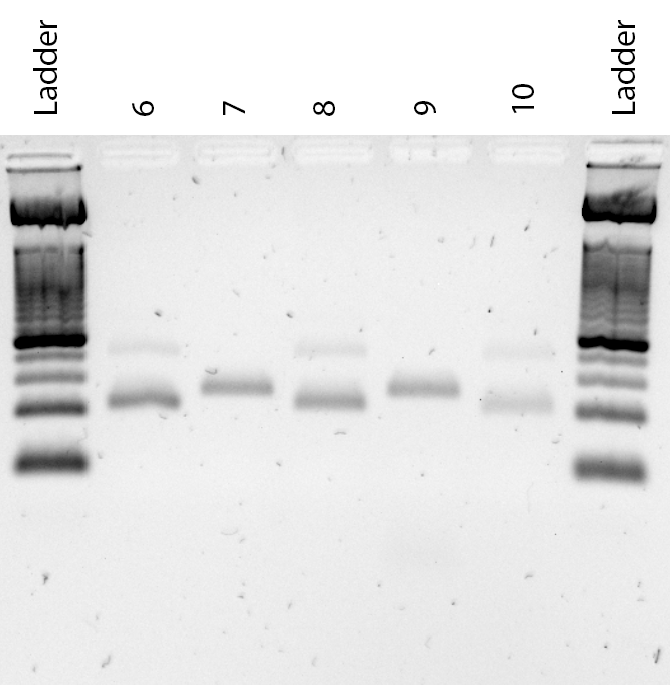
\includegraphics[width=\textwidth]{images/translator_pcr_long_1.png}
  \caption{}
  \label{translator_pcr_long_1}
\end{subfigure}
\begin{subfigure}[t]{0.47\textwidth}
  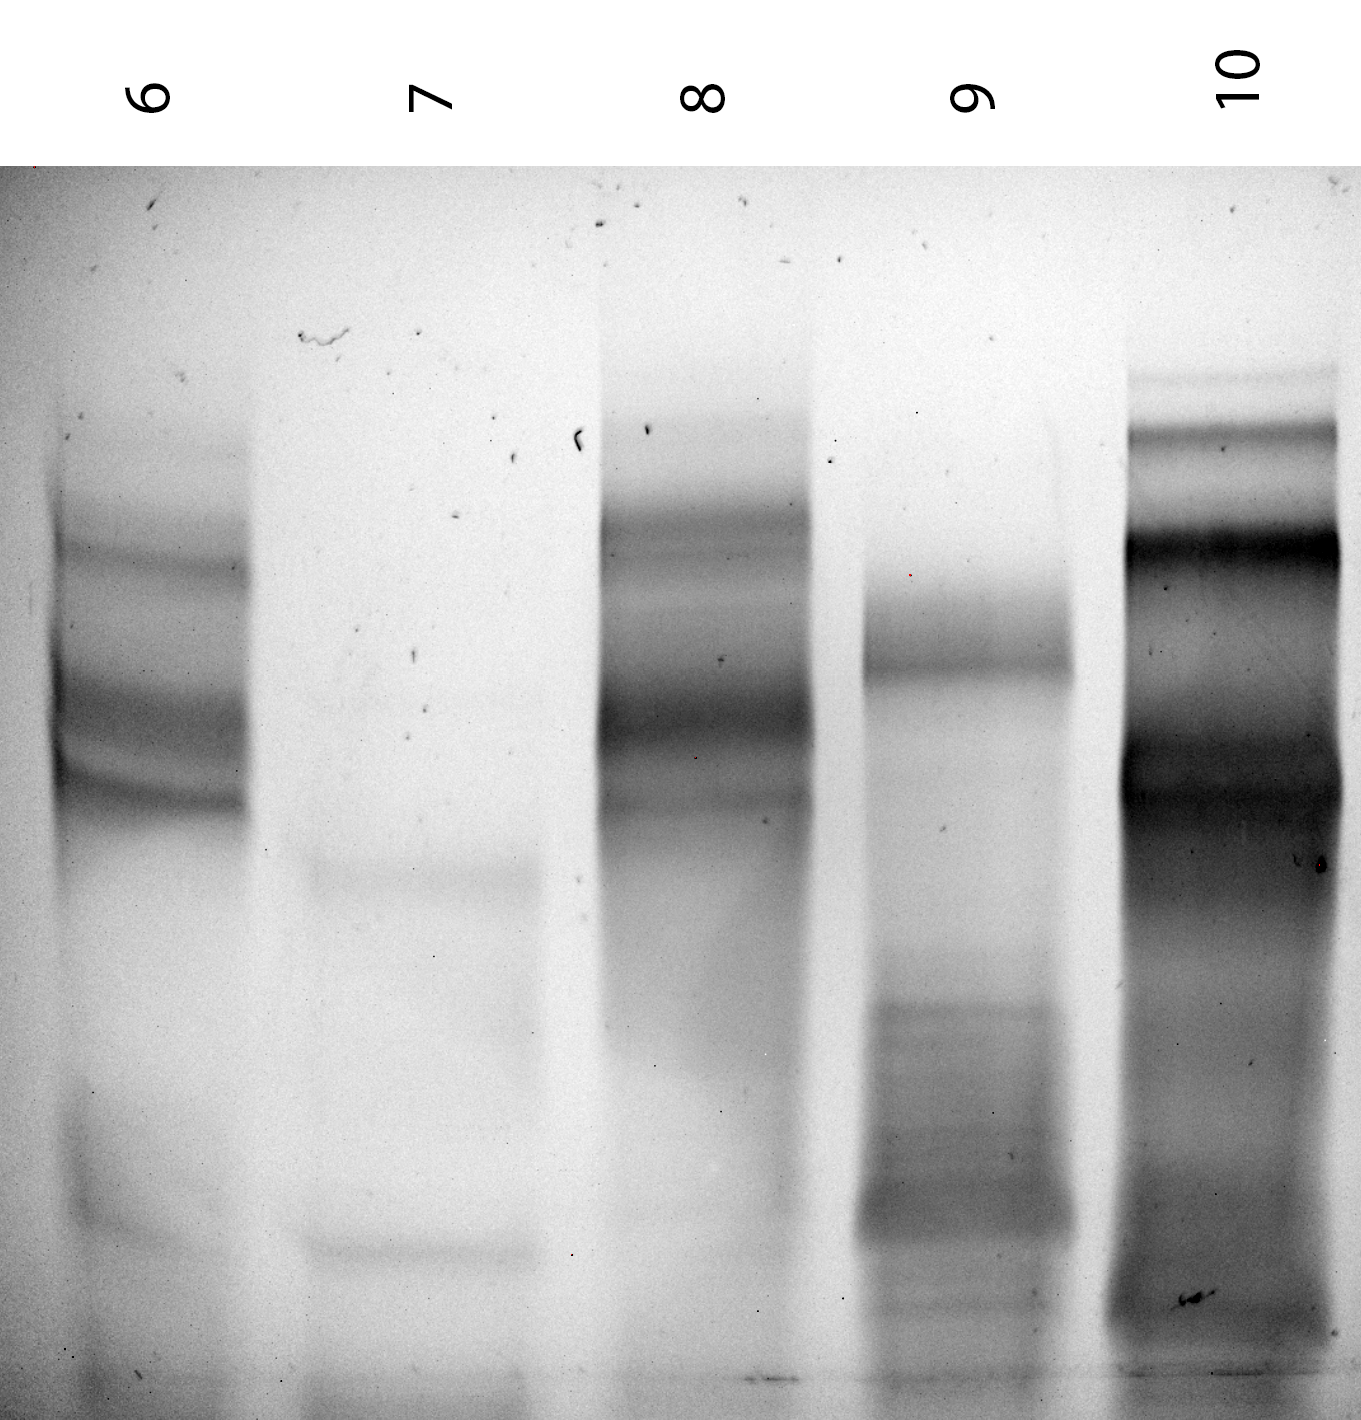
\includegraphics[width=\textwidth]{images/translator_transcription_long_ds_1.png}
  \caption{}
  \label{translator_transcription_long_ds_1}
\end{subfigure}
\caption{\subref{translator_pcr_long_1} PCR product of the long translator sequences. \subref{translator_transcription_long_ds_1} Transcription of the double-stranded long translator sequences.}
\end{figure}

The result in \fref{translator_pcr_long_1} shows the expected PCR product sizes compared with \tref{dna_strands}. Another transcription reaction was carried out on the double-stranded long translator sequences using the previous protocol. The samples were run on a 10\% denaturing PAGE gel for 2 hours at 25 W. UV shadowing still only revealed a band in strand 10, so the gel was stained with SYBR Gold and scanned.

\fref{translator_transcription_long_ds_1} shows strand 10 clearly, but still a lot of other products, and strand 7 has hardly been transcribed at all. After some further discussion with the other group members, the results can be explained by secondary structures of the RNA strands. If the strands form strong hairpins, the transcription can be aborted early, and produce unintended products. The RNA strands were checked in Nupack for secondary structures. Comparing the Nupack analysis in \fref{long_secondary_structures} with the gel in \fref{translator_transcription_long_ds_1}, the amount of product seems to follow the free energy of the secondary structure of the RNA. Strand 10 which was visible in UV shadowing has no secondary structure with the highest probability, and and strand 7 which shows the least amount of product has the lowest free energy.

The only way to avoid this problem is to create another design which doesn't have secondary structures, but since the translator sequences are locked by the desired input and output sequences, this is not a possibility. To actually get the RNA strands, they should have been ordered from IDT, synthesized and purified. This is more expensive, and was thought to be unnecessary in the beginning of the experiment. There was not enough time left to order the RNA sequences and carry out the fluorescence measurements on the reporter, so no results was obtained from the experiment.
